\begin{enumerate}[label=\bfseries Câu \arabic*:]
	\item \mkstar{1}
	
	\cauhoi{
		Trong dao động điều hòa của một vật thì tập hợp ba đại lượng nào sau đây không đổi theo thời gian?
		
		\begin{mcq}(2)
			\item Biên độ, tần số, cơ năng.
			\item Biên độ, tần số, gia tốc.
			\item Động năng, tần số, lực hồi phục.
			\item Lực hồi phục, vận tốc, cơ năng.
		\end{mcq}
	}
	\loigiai{
		\textbf{Đáp án A.}
		
		Tập hợp ba đại lượng không đổi theo thời gian: biên độ, tần số, cơ năng.
	}

	\item \mkstar{1}

\cauhoi{
	
	Trong dao động điều hòa, những đại lượng dao động cùng tần số với li độ là
	\begin{mcq}(2)
		\item động năng, thế năng và lực kéo về.
		\item vận tốc, gia tốc và lực kéo về.
		\item vận tốc, động năng và thế năng.
		\item vận tốc, gia tốc và động năng.
	\end{mcq}
}
\loigiai{
	\textbf{Đáp án B.}
	
	Trong dao động điều hòa, những đại lượng cùng tần số với li độ là: vận tốc, gia tốc, lực kéo về.
	
	Những đại lượng dao động khác tần số với li độ (cụ thể là $f'=2f$) là: động năng, thế năng.
}

	\item \mkstar{1}

\cauhoi{
	Phát biểu nào sau đây \textbf{không} đúng về dao động điều hòa?
	
	\begin{mcq}
		\item Hợp lực tác dụng vào vật có giá trị lớn nhất khi vật đi qua vị trí cân bằng.
		\item Động năng của vật biến đổi tuần hoàn với chu kì bằng một nửa chu kì dao động của vật.
		\item Tốc độ của vật lớn nhất khi vật đi qua vị trí cân bằng.
		\item Vận tốc của vật lệch pha $\xsi{0,5\pi}{rad}$ so với li độ dao động.
	\end{mcq}
}
\loigiai{
	\textbf{Đáp án A.}
	
	Dựa vào định luật II Niu-tơn:
	$$\Sigma \vec{F} = m \vec{a}.$$
	
	Tại vị trí cân bằng thì $a=0$, suy ra $\Sigma \vec{F} = 0$. Vậy hợp lực tác dụng vào vật bằng 0 khi vật đi qua vị trí cân bằng.
}

	\item \mkstar{1}

\cauhoi{
	
	Hiện tượng cộng hưởng cơ học diễn ra khi nào?
	\begin{mcq}
		\item Tần số dao động cưỡng bức bằng tần số dao động riêng của hệ.
		\item Tần số của lực cưỡng bức bé hơn tần số riêng của hệ.
		\item Tần số của lực cưỡng bức bằng tần số của dao động cưỡng bức.
		\item Tần số của lực cưỡng bức lớn hơn tần số riêng của hệ.
	\end{mcq}
}
\loigiai{
	\textbf{Đáp án A.}
	
	Hiện tượng cộng hưởng cơ học diễn ra khi tần số dao động cưỡng bức bằng tần số dao động riêng của hệ.
}

	\item \mkstar{1}

\cauhoi{
	Khi quả nặng của một con lắc đơn đi từ vị trí cân bằng đến vị trí biên thì nhận định nào dưới đây \textbf{sai}?
	
	\begin{mcq}(2)
		\item Li độ góc tăng dần.
		\item Gia tốc tăng dần.
		\item Tốc độ giảm dần.
		\item Lực căng dây tăng dần.
	\end{mcq}
}
\loigiai{
	\textbf{Đáp án D.}
	
	Khi quả nặng của một con lắc đơn đi từ vị trí cân bằng đến vị trí biên thì lực căng dây giảm.
}

	\item \mkstar{1}

\cauhoi{
	Trong dao động điều hòa, gọi $\omega$ là tần số góc, $A$ là biên độ dao động. Công thức liên hệ giữa $v$ và $x$ nào dưới đây là đúng?
	
	\begin{mcq}(2)
		\item $x^2 = \dfrac{v^2}{\omega^2} + A^2$.
		\item $\dfrac{v^2}{\omega^2} = A^2 - x^2$.
		\item $x^2 = \dfrac{\omega^2}{v^2} + A^2$.
		\item $A^2 = \dfrac{\omega^2}{v^2} + x^2$.
	\end{mcq}
}
\loigiai{
	\textbf{Đáp án B.}
	
	$$A^2 = x^2 + \dfrac{v^2}{\omega^2} \Rightarrow A^2 - x^2 = \dfrac{v^2}{\omega^2}.$$
}

	\item \mkstar{2}

\cauhoi{
	Một chất điểm dao động điều hòa theo phương trình $x=5 \cos (2\pi t + \pi)\ \text{cm}$. Quãng đường vật đi được sau $\SI{2}{s}$ là
	
	\begin{mcq}(4)
		\item $\SI{20}{cm}$.
		\item $\SI{10}{cm}$.
		\item $\SI{40}{cm}$.
		\item $\SI{80}{cm}$.
	\end{mcq}
}
\loigiai{
	\textbf{Đáp án C.}
	
	Chu kì dao động:
	$$T=\dfrac{2\pi}{\omega} = \SI{1}{s}.$$
	
	Vì $t=\SI{2}{s}=2T$ nên quãng đường vật đi được là
	$$S=2\cdot 4A = 2 \cdot 4 \cdot \SI{5}{cm} = \SI{40}{cm}.$$
}

	\item \mkstar{2}

\cauhoi{
	Một vật dao động điều hòa có biểu thức của gia tốc là $a=-100\pi^2 \cos (100 \pi t - \pi /2)\ \text{cm/s}^2$. Quãng đường vật đi được trong 1 chu kì dao động là
	
	\begin{mcq}(4)
		\item $\SI{1}{cm}$.
		\item $\SI{4}{cm}$.
		\item $\xsi{400\pi ^2}{cm}$.
		\item $\xsi{4\pi^2}{cm}$.
	\end{mcq}
}
\loigiai{
	\textbf{Đáp án B.}
	
	Dựa vào mối liên hệ giữa gia tốc cực đại và biên độ dao động, ta được:
	$$a_\text{max} = -\omega^2 A \Rightarrow A = \dfrac{-a_\text{max}}{\omega^2} = \SI{1}{cm}.$$
	
	Quãng đường vật đi được trong 1 chu kì:
	$$S=4A = \SI{4}{cm}.$$
}

	\item \mkstar{2}

\cauhoi{
	Đồ thị vận tốc-thời gian của một vật dao động điều hòa được cho như hình vẽ.
	\begin{center}
		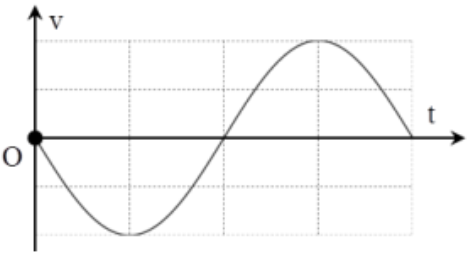
\includegraphics[scale=0.8]{../figs/VN12-2021-PH-TP007-1}
	\end{center}

	Mốc thời gian đã được chọn vào lúc
	\begin{mcq}
		\item vật đi qua vị trí cân bằng theo chiều âm.
		\item vật đi qua vị trí cân bằng theo chiều dương.
		\item vật ở biên âm.
		\item vật ở biên dương.
	\end{mcq}
}
\loigiai{
	\textbf{Đáp án D.}
	
	Dựa vào đồ thị, tại thời điểm $t=0$ thì $v=0$ và có xu hướng về phía vận tốc âm. Đó là thời điểm mà vật ở vị trí biên dương.
}

	\item \mkstar{2}

\cauhoi{
	Khoảng thời gian liên tiếp để động năng và thế năng của một vật dao động điều hòa bằng nhau là $\SI{0.3}{s}$. Chu kì dao động của vật là
	
	\begin{mcq}(4)
		\item $\SI{0.3}{s}$.
		\item $\SI{0.6}{s}$.
		\item $\SI{0.9}{s}$.
		\item $\SI{1.2}{s}$.
	\end{mcq}
}
\loigiai{
	\textbf{Đáp án D.}
	
	Khoảng thời gian liên tiếp giữa hai lần động năng bằng thế năng là $T/4$:
	$$\dfrac{T}{4} = \SI{0.3}{s} \Rightarrow T = \SI{1.2}{s}.$$
}

	\item \mkstar{2}

\cauhoi{
	Một vật dao động điều hòa với biên độ $A$ và cơ năng $W$. Chọn mốc thế năng tại vị trí cân bằng. Khi vật đi qua vị trí có li độ $x=2A/3$ thì động năng của vật là
	
	\begin{mcq}(4)
		\item $\dfrac{5}{9}W$.
		\item $\dfrac{4}{9} W$.
		\item $\dfrac{7}{9} W$.
		\item $\dfrac{2}{9} W$.
	\end{mcq}
}
\loigiai{
	\textbf{Đáp án A.}
	
	Lập tỉ lệ:
	$$\dfrac{W_\text{đ}}{W} = \dfrac{A^2 - x^2}{A^2} = \dfrac{5}{9}.$$
}

	\item \mkstar{2}

\cauhoi{
	Tiến hành thí nghiệm đo gia tốc trọng trường $g$ bằng con lắc đơn, một học sinh đo được chiều dài con lắc là $l = \bar{l} \pm \Delta l$ (đơn vị m). Chu kì dao động nhỏ của nó là $T=\bar{T} \pm \Delta T$ (đơn vị s). Bỏ qua sai số của $\pi$, biểu thức sai số của $g$ là
	
	\begin{mcq}(2)
		\item $\dfrac{\Delta g}{\bar{g}} = \dfrac{\Delta T}{\bar{T}} + \dfrac{2 \Delta l}{\bar{l}}$.
		\item $\dfrac{\Delta g}{\bar{g}} = \dfrac{\Delta T}{\bar{T}} + \dfrac{\Delta l}{\bar{l}}$.
		\item $\dfrac{\Delta g}{\bar{g}} = \dfrac{2\Delta T}{\bar{T}} + \dfrac{2 \Delta l}{\bar{l}}$.
		\item $\dfrac{\Delta g}{\bar{g}} = \dfrac{2\Delta T}{\bar{T}} + \dfrac{\Delta l}{\bar{l}}$.
	\end{mcq}
}
\loigiai{
	\textbf{Đáp án D.}
	
	Biểu thức xác định $g$:
	$$g=\left(\dfrac{2\pi}{T}\right)^2 l \Rightarrow \dfrac{\Delta g}{\bar{g}} = \dfrac{2\Delta T}{\bar{T}} + \dfrac{\Delta l}{\bar{l}}$$
}

	\item \mkstar{2}

\cauhoi{
	Một vật nhỏ khối lượng $\SI{100}{g}$ dao động điều hòa trên một quỹ đạo thẳng dài $\SI{20}{cm}$ với tần số góc $\SI{6}{rad/s}$. Cơ năng của vật này là
	
	\begin{mcq}(4)
		\item $\SI{0.036}{J}$.
		\item $\SI{0.018}{J}$.
		\item $\SI{18}{J}$.
		\item $\SI{36}{J}$.
	\end{mcq}
}
\loigiai{
	\textbf{Đáp án B.}
	
	Tính biên độ dao động dựa vào chiều dài quỹ đạo:
	$$A=\dfrac{L}{2} = \SI{10}{cm}.$$
	
	Cơ năng của vật:
	$$W=\dfrac{1}{2} m \omega^2 A^2 = \SI{0.018}{J}.$$
}

	\item \mkstar{2}

\cauhoi{
	Một vật nhỏ khối lượng $m=\SI{0.01}{kg}$ treo ở đầu một lò xo có độ cứng $k=\SI{4}{N/m}$, dao động điều hòa quanh vị trí cân bằng. Chu kì dao động của vật là
	
	\begin{mcq}(4)
		\item $\SI{0.624}{s}$.
		\item $\SI{0.314}{s}$.
		\item $\SI{0.196}{s}$.
		\item $\SI{0.157}{s}$.
	\end{mcq}
}
\loigiai{
	\textbf{Đáp án B.}
	
	Chu kì dao động:
	$$T=2\pi \sqrt{\dfrac{m}{k}} = \SI{0.0314}{s}.$$
}

	\item \mkstar{2}

\cauhoi{
	Một vật nặng treo vào đầu lò xo làm cho lò xo dãn ra $\SI{4}{cm}$, đầu kia treo vào một điểm O cố định. Hệ dao động điều hòa theo phương thẳng đứng. Cho $g=\xsi{\pi^2}{m/s^2}$. Chu kì dao động của hệ là
	
	\begin{mcq}(4)
		\item $\SI{0.8}{s}$.
		\item $\SI{0.4}{s}$.
		\item $\SI{0.2}{s}$.
		\item $\SI{1.6}{s}$.
	\end{mcq}
}
\loigiai{
	\textbf{Đáp án B.}
	
	Chu kì của dao động là
	$$T=2\pi \sqrt{\dfrac{\Delta l}{g}} = \SI{0.4}{s}.$$
}

	\item \mkstar{2}

\cauhoi{
	Một con lắc lò xo gồm lò xo có độ cứng $k=\SI{100}{N/m}$ và vật nặng có khối lượng $m$, dao động điều hòa quanh trục O$x$ nằm ngang. Thế năng của con lắc khi vật đi qua vị trí có li độ $x=\SI{3}{cm}$ theo chiều âm là
	
	\begin{mcq}(4)
		\item $\SI{0.045}{J}$.
		\item $\SI{0.09}{J}$.
		\item $\SI{-0.045}{J}$.
		\item $\SI{-0.09}{J}$.
	\end{mcq}
}
\loigiai{
	\textbf{Đáp án A.}
	
	Thế năng của con lắc khi vật ở vị trí $x=\SI{3}{cm}$:
	$$W_\text{t} = \dfrac{1}{2} kx^2 = \SI{0.045}{J}.$$
}

	\item \mkstar{2}

\cauhoi{
	Một con lắc lò xo dao động điều hòa với biên độ $A=\SI{10.0}{cm}$ và cơ năng $\SI{0.8}{J}$. Độ cứng của lò xo là
	
	\begin{mcq}(4)
		\item $\SI{80}{N/m}$.
		\item $\SI{40}{N/m}$.
		\item $\SI{1.6}{N/m}$.
		\item $\SI{160}{N/m}$.
	\end{mcq}
}
\loigiai{
	\textbf{Đáp án D.}
	
	Áp dụng biểu thức của cơ năng:
	$$W=\dfrac{1}{2} kA^2 \Rightarrow k = \SI{160}{N/m}.$$
}

	\item \mkstar{2}

\cauhoi{
	Một vật tham gia đồng thời hai dao động điều hòa cùng phương có phương trình lần lượt là $x_1=3\cos \left(10 \pi t + \dfrac{\pi}{6}\right)\ \text{cm}$ và $x_2 = 7 \cos \left(10 \pi t + \dfrac{13\pi}{6}\right)\ \text{cm}$. Dao động tổng hợp có phương trình là
	
	\begin{mcq}(2)
		\item $x=10 \cos \left(10 \pi t + \dfrac{7\pi}{3}\right)\ \text{cm}$.
		\item $x=4 \cos \left(10 \pi t + \dfrac{\pi}{6}\right)\ \text{cm}$.
		\item $x=10 \cos \left(20 \pi t + \dfrac{\pi}{6}\right)\ \text{cm}$.
		\item $x=10 \cos \left(10 \pi t + \dfrac{\pi}{6}\right)\ \text{cm}$.
	\end{mcq}
}
\loigiai{
	\textbf{Đáp án D.}
	
	Phương trình dao động tổng hợp:
	$$x=10 \cos \left(10 \pi t + \dfrac{\pi}{6}\right)\ \text{cm}$$
}

	\item \mkstar{2}

\cauhoi{
	Một con lắc lò xo có độ cứng $k$ treo thẳng đứng, đầu trên gắn cố định, đầu dưới treo quả cầu nhỏ ở nơi có gia tốc trọng trường $g$. Khi vật ở vị trí cân bằng, lò xo có độ dãn $\Delta l$. Cho con lắc dao động điều hòa theo phương thẳng đứng với biên độ $A$ (với $A> \Delta l$). Lực đàn hồi cực tiểu của lò xo được xác định bởi biểu thức nào sau đây?
	
	\begin{mcq}(2)
		\item $F_\text{đh min} = k A$.
		\item $F_\text{đh min} = k(A - \Delta l)$.
		\item $F_\text{đh min} = 0$.
		\item $F_\text{đh min} = k (\Delta l - A)$.
	\end{mcq}
}
\loigiai{
	\textbf{Đáp án C.}
	
	Khi $A<\Delta l$ thì $F_\text{đh min} = k (\Delta l - A)$.
	
	Khi $A>\Delta l$ thì $F_\text{đh min} = 0$.
}

	\item \mkstar{3}

\cauhoi{
	Tỉ số giữa gia tốc của một vật dao động điều hòa so với gia tốc cực đại tại vị trí động năng gấp 2 lần thế năng là
	
	\begin{mcq}(4)
		\item $\dfrac{1}{2}$.
		\item $\dfrac{1}{\sqrt{2}}$.
		\item $\dfrac{1}{3}$.
		\item $\dfrac{1}{\sqrt{3}}$.
	\end{mcq}
}
\loigiai{
	\textbf{Đáp án D.}
	
	Ta có tỉ số:
	$$\dfrac{W_\text{đ}}{W_\text{t}} = 2 \Rightarrow \dfrac{A^2 - x^2}{x^2} = 2 \Rightarrow |x| = \dfrac{A}{\sqrt{3}} \Rightarrow a = \dfrac{a_\text{max}}{\sqrt{3}}.$$
}

	\item \mkstar{3}

\cauhoi{
	Một vật dao động điều hòa theo phương trình $x=2 \cos (\pi t - \pi /3)\ \text{cm}$, trong đó $t$ tính bằng giây. Tính từ lúc $t=0$, thời điểm vật đi qua vị trí có thế năng bằng 3 lần động năng lần thứ 2018 là
	
	\begin{mcq}(4)
		\item $\SI{1008.5}{s}$.
		\item $\SI{1009.5}{s}$.
		\item $\SI{1008}{s}$.
		\item $\SI{1009}{s}$.
	\end{mcq}
}
\loigiai{
	\textbf{Đáp án A.}
	
	Tại thời điểm $t=0$, vật ở vị trí $x=A \cos (-\dfrac{\pi}{3}) = \dfrac{A}{2}$, theo chiều dương.
	
	Vị trí mà vật có thế năng gấp 3 lần động nặng là $x=\dfrac{A\sqrt{3}}{2}$.
	
	Ta nhận thấy 2016 chia hết cho 4 (vì 1 chu kì có 4 lần thế năng gấp 3 lần động năng), nên ta phân tích lần thứ 2018 thành $2+2016$, nghĩa là phân tích thành 2 lần đầu và 2016 lần sau.
	
	Lần thứ nhất mà vật có thế năng gấp 3 lần động năng là thời điểm:
	$$t_1 = \dfrac{T}{6} - \dfrac{T}{12} = \dfrac{T}{12}.$$
	
	Lần thứ hai mà vật có thế năng gấp 3 lần động năng là thời điểm:
	$$t_2 = t_1 + 2 \cdot \dfrac{T}{12} = \dfrac{3T}{12}.$$
	
	Lần thứ 2018 mà vật có thế năng gấp 3 lần động năng là thời điểm:
	$$t_{2018} = t_2 + \dfrac{2016}{4} T = \dfrac{3T}{12} + 504T = \SI{1008.5}{s}.$$
	}

	\item \mkstar{3}

\cauhoi{
	Một chất điểm dao động điều hòa trên trục O$x$ với biên độ $\SI{10}{cm}$, chu kì $\SI{2}{s}$. Mốc thế năng ở VTCB. Tốc độ trung bình của chất điểm trong khoảng thời gian ngắn nhất khi chất điểm đi từ vị trí có động năng bằng 3 lần thế năng đến vị trí có động năng bằng $1/3$ lần thế năng là
	
	\begin{mcq}(4)
		\item $\SI{7.32}{cm/s}$.
		\item $\SI{21.96}{cm/s}$.
		\item $\SI{14.64}{cm/s}$.
		\item $\SI{26.12}{cm/s}$.
	\end{mcq}
}
\loigiai{
	\textbf{Đáp án B.}
	
	Quãng đường vật đi được:
	$$S=\dfrac{A\sqrt{3}}{2} - \dfrac{A}{2} = \xsi{-5+5\sqrt{3}}{cm}.$$
	
	Thời gian để đi hết quãng đường đó:
	$$t=\dfrac{T}{6} - \dfrac{T}{12} = \dfrac{T}{12} = \xsi{\dfrac{1}{6}}{s}.$$
	
	Vận tốc trung bình:
	$$v=\dfrac{S}{t} = \SI{21.96}{cm/s}$$
}

	\item \mkstar{3}

\cauhoi{
	Một vật nhỏ dao động điều hòa dọc theo trục O$x$. Khi vật cách vị trí cân bằng một đoạn $\SI{2}{cm}$ thì động năng của vật là $\SI{0.48}{J}$. Khi vật cách vị trí cân bằng một đoạn $\SI{6}{cm}$ thì động năng của vật là $\SI{0.32}{J}$. Biên độ dao động của vật bằng
	
	\begin{mcq}(4)
		\item $\SI{8}{cm}$.
		\item $\SI{14}{cm}$.
		\item $\SI{10}{cm}$.
		\item $\SI{12}{cm}$.
	\end{mcq}
}
\loigiai{
	\textbf{Đáp án B.}
	
	Vì cơ năng không đổi theo thời gian nên ta có:
	$$W_1 = W_2 \Rightarrow W_\text{đ1} + W_\text{t1} = W_\text{đ2} + W_\text{t2} \Rightarrow \dfrac{1}{2} m\omega^2 x_1^2 + \SI{0.48}{J} = \dfrac{1}{2} m \omega^2 x_2^2 + \SI{0.32}{J} \Rightarrow m \omega^2 = 100.$$
	
	Tính được cơ năng của vật:
	$$W=\dfrac{1}{2} m \omega^2 x_1^2 + W_\text{đ1} = \SI{0.5}{J}.$$
	
	Suy ra biên độ dao động là
	$$A=\sqrt{\dfrac{W}{\dfrac{1}{2} m \omega^2}} = \SI{10}{cm}.$$
}

	\item \mkstar{3}

\cauhoi{
	Một vật dao động điều hòa với tần số $f=\SI{3}{Hz}$. Tại thời điểm $t=\SI{1.5}{s}$, vật có li độ $x=\SI{4}{cm}$ và vận tốc $v=\xsi{24\pi \sqrt{3}}{cm/s}$ đang hướng về vị trí cân bằng. Phương trình dao động của vật là
	
	\begin{mcq}(2)
		\item $x= 8 \cos \left(6 \pi t - \dfrac{2\pi}{3}\right)\ \text{cm}$.
		\item $x= 8 \cos \left(6 \pi t - \dfrac{\pi}{3}\right)\ \text{cm}$.
		\item $x= 4\sqrt{3} \cos \left(6 \pi t + \dfrac{2\pi}{3}\right)\ \text{cm}$.
		\item $x= 4\sqrt{3} \cos \left(6 \pi t - \dfrac{\pi}{3}\right)\ \text{cm}$.
	\end{mcq}
}
\loigiai{
	\textbf{Đáp án A.}
	
	Tần số góc của dao động:
	$$\omega = 2\pi f = \xsi{6\pi}{rad/s}.$$
	
	Áp dụng hệ thức độc lập để xác định biên độ:
	$$A=\sqrt{x^2 + \dfrac{v^2}{\omega^2}} = \SI{8}{cm}.$$
	
	Khi đó, $x=\dfrac{A}{2}$ và vật đang hướng về vị trí cân bằng, nên pha của dao động là $\varphi_2 = \dfrac{\pi}{3}\ \text{rad}$.
	
	Trước đó $\SI{1.5}{s}=\SI{4.5}{} T$ chính là thời điểm ban đầu, tìm được pha ban đầu là
	$$\varphi = \dfrac{\pi}{3}\ \text{rad}-\xsi{9\pi}{rad} = \dfrac{-26\pi}{3}\ \text{rad}=\dfrac{-2\pi}{3}\ \text{rad}.$$
	
	Vậy phương trình dao động là $x=8 \cos \left(6\pi t - \dfrac{2\pi}{3}\right)\ \text{cm}$.
}

	\item \mkstar{3}

\cauhoi{
	Một con lắc lò xo gồm một quả cầu nhỏ gắn vào đầu một lò xo, dao động điều hòa với biên độ $\SI{2.5}{cm}$ dọc theo trục O$x$, với chu kì $\SI{1.2}{s}$. Vào thời điểm $t=0$, quả cầu đi qua vị trí cân bằng theo chiều dương của trục O$x$. Hỏi vào thời điểm nào sau đây quả cầu có li độ $x=\SI{1.25}{cm}$?
	
	\begin{mcq}(4)
		\item $t=\SI{0.04}{s}$.
		\item $t=\SI{0.75}{s}$.
		\item $t=\SI{0.5}{s}$.
		\item $t=\SI{0.6}{s}$.
	\end{mcq}
}
\loigiai{
	\textbf{Đáp án C.}
	
	Tần số góc của dao động:
	$$\omega = \dfrac{2\pi}{T} = \xsi{\dfrac{5\pi}{3}}{rad/s}.$$
	
	Pha ban đầu: $\varphi = \xsi{\dfrac{-\pi}{2}}{rad}$.
	
	Phương trình dao động:
	$$x=\SI{2.5}{} \cos \left(\dfrac{5\pi}{3} t - \dfrac{\pi}{2}\right)\ \text{cm}.$$
	
	Với $x=\SI{1.25}{cm}$ thì $t=\SI{0.5}{s}$.
}

	\item \mkstar{3}

\cauhoi{
	Một đầu của một lò xo được treo vào điểm cố định O, đầu kia treo một quả nặng $m_1$ thì vật dao động với chu kì $T_1 = \SI{0.6}{s}$. Khi thay vật $m_1$ thành vật $m_2$ thì vật dao động với chu kì $T_2=\SI{0.8}{s}$. Chu kì dao động khi treo đồng thời $m_1$ và $m_2$ vào lò xo là
	
	\begin{mcq}(4)
		\item $T=\SI{1.6}{s}$.
		\item $T=\SI{1.4}{s}$.
		\item $T=\SI{1.0}{s}$.
		\item $T=\SI{1.2}{s}$.
	\end{mcq}
}
\loigiai{
	\textbf{Đáp án C.}
	
	Ta có công thức tính chu kì:
	$$T=2\pi \sqrt{\dfrac{m}{k}} \Rightarrow m \sim T^2.$$
	
	Chu kì khi treo đồng thời $m_1$ và $m_2$:
	$$T^2 = T_1^2 + T_2^2 \Rightarrow T=\SI{1.0}{s}.$$
}

	\item \mkstar{3}

\cauhoi{
	Một chất điểm dao động điều hòa trên trục O$x$. Trong thời gian $\SI{31.4}{s}$ chất điểm thực hiện được 100 dao động toàn phần. Gốc thời gian là lúc chất điểm đi qua vị trí có li độ $\SI{2}{cm}$ theo chiều âm với tốc độ là $\xsi{40\sqrt{3}}{cm/s^2}$. Lấy $\pi = \SI{3.14}{}$. Phương trình dao động của chất điểm là
	
	\begin{mcq}(2)
		\item $x= 6 \cos \left(20 t - \dfrac{\pi}{6}\right)\ \text{cm}$.
		\item $x=4 \cos \left(20 t + \dfrac{\pi}{3}\right)\ \text{cm}$.
		\item $x= 4\cos \left(20 t - \dfrac{\pi}{3}\right)\ \text{cm}$.
		\item $x=6 \cos \left(20 t + \dfrac{\pi}{6}\right)\ \text{cm}$.
	\end{mcq}
}
\loigiai{
	\textbf{Đáp án B.}
	
	Ta có:
	$$T=\dfrac{\Delta t}{n} = \SI{0.314}{s} \Rightarrow \omega = \SI{20}{rad/s}.$$
	
	Biên độ dao động:
	$$A=\sqrt{x_0^2 + \left(\dfrac{v_0}{\omega}\right)^2} = \SI{4}{cm}.$$
	
	Khi $t=0$ thì $x_0 = \pm \SI{2}{cm}$ và $v<0$. Nên pha ban đầu:
	$$\varphi_0 = \dfrac{\pi}{3}\ \text{rad}.$$
	
	Phương trình dao động của chất điểm là
	$$x=4 \cos \left(20 t + \dfrac{\pi}{3}\right)\ \text{cm}.$$
}

	\item \mkstar{3}

\cauhoi{
	Một chất điểm dao động điều hòa có phương trình $x=6 \cos \left(10t - \dfrac{\pi}{2}\right)\ \text{cm}$. Vận tốc của chất điểm có phương trình
	
	\begin{mcq}(2)
		\item $v=-60 \cos (10t)\ \text{cm/s}$.
		\item $v=60 \cos \left(10t - \dfrac{\pi}{2}\right)\ \text{cm/s}$.
		\item $v=60 \cos (10t)\ \text{cm/s}$.
		\item $v=60 \cos \left(10t + \dfrac{\pi}{2}\right)\ \text{cm/s}$.
	\end{mcq}
}
\loigiai{
	\textbf{Đáp án C.}
	
	Phương trình vận tốc:
	$$v=x'=-60 \sin \left(10t - \dfrac{\pi}{2}\right) = 60 \cos (10t)\ \text{cm/s}.$$
}

	\item \mkstar{3}

\cauhoi{
	Một vật treo vào lò xo làm nó dãn ra $\SI{4}{cm}$. Cho $g=\xsi{\pi^2}{m/s^2}$. Biết lực đàn hồi cực đại và cực tiểu trong quá trình dao động lần lượt là $\SI{10}{N}$ và $\SI{6}{N}$. Chiều dài tự nhiên của lò xo là $\SI{20}{cm}$. Chiều dài cực đại và cực tiểu của lò xo trong quá trình dao động là
	
	\begin{mcq}(2)
		\item $\SI{25}{cm}$ và $\SI{24}{cm}$.
		\item $\SI{24}{cm}$ và $\SI{23}{cm}$.
		\item $\SI{26}{cm}$ và $\SI{24}{cm}$.
		\item $\SI{25}{cm}$ và $\SI{23}{cm}$.
	\end{mcq}
}
\loigiai{
	\textbf{Đáp án D.}
	
	Lập tỉ lệ:
	$$\dfrac{F_\text{đh max}}{F_\text{đh min}} = \dfrac{k(\Delta l + A)}{k (\Delta l - A)} = \dfrac{10}{6} \Rightarrow A = \SI{1}{cm}.$$
	
	Chiều dài cực đại:
	$$l_\text{max} = l_0 + \Delta l + A = \SI{25}{cm}.$$
	
	Chiều dài cực tiểu:
	$$l_\text{min} = l_0 + \Delta l - A = \SI{23}{cm}.$$
}

	\item \mkstar{3}

\cauhoi{
	Một con lắc lò xo dao động với phương trình $x=10 \cos \left(20 t - \dfrac{\pi}{3}\right)\ \text{cm}$. Biết vật nặng có khối lượng $m=\SI{100}{g}$. Thế năng của con lắc tại thời điểm $t=\pi\ \text{(s)}$ là
	
	\begin{mcq}(4)
		\item $\SI{0.25}{J}$.
		\item $\SI{0.5}{J}$.
		\item $\SI{0.5}{mJ}$.
		\item $\SI{0.05}{J}$.
	\end{mcq}
}
\loigiai{
	\textbf{Đáp án D.}
	
	Li độ của vật tại thời điểm $t=\xsi{\pi}{s}$:
	$$x = 10 \cos \left(20t - \dfrac{\pi}{3}\right)\ \text{cm} = 10 \cos \left(20 \pi - \dfrac{\pi}{3}\right)\ \text{cm} = \SI{5}{cm}.$$
	
	Thế năng khi đó là
	$$W_\text{t} = \dfrac{1}{2} m \omega^2 x^2 = \SI{0.05}{J}.$$
}

	\item \mkstar{3}

\cauhoi{
	Một vật dao động điều hòa theo phương trình $x = 20 \cos (2\pi t + \pi)\ \text{cm}$. Thời điểm vật đi qua vị trí có li độ $x=\xsi{10\sqrt{2}}{cm}$ theo chiều âm là
	
	\begin{mcq}(4)
		\item $\xsi{\dfrac{5}{8}}{s}$.
		\item $\xsi{\dfrac{14}{8}}{s}$.
		\item $\xsi{\dfrac{8}{7}}{s}$.
		\item $\xsi{\dfrac{8}{14}}{s}$.
	\end{mcq}
}
\loigiai{
	\textbf{Đáp án A.}
	
	Ta có $T=\dfrac{2\pi}{\omega} = \SI{1}{s}$, $x=\dfrac{A\sqrt{2}}{2}$.
	
	Tại thời điểm $t=0$, vật ở vị trí biên âm. Thời điểm để vật đi qua vị trí có li độ $x=\dfrac{A\sqrt{2}}{2}$ theo chiều âm là
	$$t=\dfrac{T}{2} + \dfrac{T}{8} = \xsi{\dfrac{5}{8}}{s}.$$
}

	\item \mkstar{3}

\cauhoi{
	Hai lò xo có độ cứng lần lượt là $k_1$, $k_2$ và có cùng độ dài. Một vật nặng khi treo vào lò xo $k_1$ thì vật dao động với chu kì $T_1=\SI{0.3}{s}$, còn khi treo vào lò xo $k_2$ thì dao động với chu kì $T_2=\SI{0.4}{s}$. Ghép song song hai lò xo đó với nhau rồi treo vật nói trên vào thì vật dao động với chu kì
	
	\begin{mcq}(4)
		\item $\SI{0.5}{s}$.
		\item $\SI{0.24}{s}$.
		\item $\SI{0.36}{s}$.
		\item $\SI{0.48}{s}$.
	\end{mcq}
}
\loigiai{
	\textbf{Đáp án B.}
	
	Khi ghép song song 2 lò xo thì độ cứng tương đương của hệ là
	$$k=k_1 + k_2$$
	
	Mà $T=2\pi \sqrt{\dfrac{m}{k}} \Rightarrow k \sim \dfrac{1}{T^2}$. Suy ra:
	$$\dfrac{1}{T^2} = \dfrac{1}{T_1^2} + \dfrac{1}{T_2^2} \Rightarrow T = \SI{0.24}{s}.$$
}

	\item \mkstar{3}

\cauhoi{
	Một vật tham gia đồng thời hai dao động điều hòa cùng phương, cùng tần số, cùng biên độ $A$ và lệch pha nhau $\xsi{\dfrac{\pi}{2}}{rad}$. Biên độ dao động tổng hợp của hai dao động trên bằng
	
	\begin{mcq}(4)
		\item $A$.
		\item $A\sqrt{2}$.
		\item $2A$.
		\item $2\sqrt{A}$.
	\end{mcq}
}
\loigiai{
	\textbf{Đáp án B.}
	
	Vì hai dao động thành phần vuông pha nên:
	$$A' = \sqrt{A^2 + A^2} = A \sqrt{2}.$$
}

	\item \mkstar{3}

\cauhoi{
	Một con lắc lò xo gồm lò xo có độ cứng $k=\SI{30}{N/m}$ và vật nặng có khối lượng $\SI{0.3}{kg}$ dao động điều hòa. Tại thời điểm $t$, vận tốc và gia tốc của vật là $\SI{40}{cm/s}$ và $\SI{3}{m/s^2}$. Biên độ dao động của vật là
	
	\begin{mcq}(4)
		\item $\SI{5}{cm}$.
		\item $\SI{25}{cm}$.
		\item $\SI{2.5}{cm}$.
		\item $\SI{0.25}{cm}$.
	\end{mcq}
}
\loigiai{
	\textbf{Đáp án A.}
	
	Tần số góc của dao động:
	$$\omega = \sqrt{\dfrac{k}{m}} = \SI{10}{rad/s}.$$
	
	Ta có công thức liên hệ giữa $a$ và $x$ là
	$$a=-\omega^2 x \Rightarrow x = \SI{-3}{cm}.$$
	
	Áp dụng hệ thức độc lập để tính $A$:
	$$A=\sqrt{x^2 + \dfrac{v^2}{\omega^2}} = \SI{5}{cm}.$$
}

	\item \mkstar{3}

\cauhoi{
	Một vật tham gia đồng thời hai dao động điều hòa cùng phương, cùng tần số, với các phương trình $x_1 = 3 \cos (\omega t)\ \text{cm}$, $x_2 = 3 \sin (\omega t + \pi)\ \text{cm}$. Phương trình dao động tổng hợp của vật là
	
	\begin{mcq}(2)
		\item $x=3\sqrt{2} \cos \left(\omega t + \dfrac{3\pi}{4}\right)\ \text{cm}$.
		\item $x=3\sqrt{2}\cos (\omega t + \pi)\ \text{cm}$.
		\item $x=3\sqrt{2}\cos \left(\omega t + \dfrac{\pi}{4}\right)\ \text{cm}$.
		\item $x=3\cos \left(\omega t + \dfrac{\pi}{4}\right)\ \text{cm}$.
	\end{mcq}
}
\loigiai{
	\textbf{Đáp án C.}
	
	Áp dụng quy tắc biến đổi lượng giác: $\sin (\varphi) = \cos (\varphi - \dfrac{\pi}{2})$. Ta được:
	$$x_2 = 3 \cos \left(\omega t + \dfrac{\pi}{2}\right)\ \text{cm}.$$
	
	Phương trình dao động tổng hợp:
	$$x=3\sqrt{2} \cos \left(\omega t + \dfrac{\pi}{4}\right)\ \text{cm}.$$
}

	\item \mkstar{4}

\cauhoi{
	Vật dao động điều hòa có vận tốc cực đại bằng $\SI{3}{m/s}$ và gia tốc cực đại bằng $\xsi{30\pi}{m/s^2}$. Thời điểm ban đầu vật có vận tốc $\SI{1.5}{m/s}$ và thế năng đang tăng. Hỏi vào thời điểm nào sau đây vật có gia tốc bằng $\xsi{15 \pi}{m/s^2}$?
	
	\begin{mcq}(4)
		\item $\SI{0.20}{s}$.
		\item $\SI{0.05}{s}$.
		\item $\SI{0.10}{s}$.
		\item $\SI{0.15}{s}$.
	\end{mcq}
}
\loigiai{
	\textbf{Đáp án D.}
	
	Lập tỉ số:
	$$\dfrac{a_\text{max}}{v_\text{max}} = \dfrac{\omega^2 A}{\omega A} = \omega = \dfrac{30\pi}{3} = \xsi{10\pi}{rad/s} \Rightarrow A = \dfrac{3}{10\pi}\ \text{m}.$$
	
	Tại thời điểm ban đầu, $v_0 = \dfrac{v_\text{max}}{2}$ nên $|x_0| = \dfrac{A\sqrt{3}}{2}$.
	
	Mà thế năng đang tăng, kết hợp với $v_0$ nên $x_0 >0$, hay $x_0 = \dfrac{A\sqrt{3}}{2}$. Khi đó $\varphi = \dfrac{\pi}{6}\ \text{rad}$. Suy ra:
	$$a=-30\pi \cos (10\pi t - \pi /6)\ \text{m/s}^2.$$
	
	Vật có gia tốc $a=\xsi{15\pi}{m/s^2}$ tại thời điểm $t=\dfrac{1}{12} + \dfrac{k}{5}$ hoặc $t=\dfrac{-1}{20} + \dfrac{k}{5}$.
	
	Thay bốn đáp án vào thì thấy $t=\SI{0.15}{s}$ thỏa mãn.
}

	\item \mkstar{4}

\cauhoi{
	Hai vật dao động điều hòa dọc theo các trục song song với nhau. Phương trình dao động của các vật lần lượt là $x_1 = 3 \cos \left(5\pi t - \dfrac{\pi}{3}\right)$ và $x_2 = \sqrt{3}\cos \left(5\pi t - \dfrac{\pi}{6}\right)$ ($x$ tính bằng cm; $t$ tính bằng s). Trong khoảng thời gian $\SI{1}{s}$ đầu tiên thì hai vật có cùng li độ mấy lần?
	
	\begin{mcq}(4)
		\item 2 lần.
		\item 3 lần.
		\item 5 lần.
		\item 6 lần.
	\end{mcq}
}
\loigiai{
	\textbf{Đáp án D.}
	
	Ta thấy hai vật gặp nhau tại thời điểm ban đầu ($t_1=0$) nên:
	$$x_1 = x_2 = \dfrac{3}{2}\ \text{cm}.$$
	
	Chu kì $T=\dfrac{2\pi}{\omega} = \SI{0.4}{s}$.
	
	Trong $\SI{1}{s}$ có $t=(n-1) \dfrac{T}{2} + t_1 \Rightarrow n = 6$ lần.
}

	\item \mkstar{4}

\cauhoi{
	Một con lắc lò xo đang dao động tắt dần. Người ta đo được độ giảm tương đối của biên độ trong hai chu kì đầu tiên là $\SI{7.5}{\percent}$. Độ giảm cơ năng tương ứng là
	
	\begin{mcq}(4)
		\item $\SI{14}{\percent}$.
		\item $\SI{92.5}{\percent}$.
		\item $\SI{9.25}{\percent}$.
		\item $\SI{0.86}{\percent}$.
	\end{mcq}
}
\loigiai{
	\textbf{Đáp án A.}
	
	Độ giảm tương đối của biên độ là $\dfrac{\Delta A}{A_0} = \SI{7.5}{\percent}$, suy ra $\Delta A = \SI{0.075}{} A_0$.
	
	Mà $\Delta A = A_0 - A_1 \Rightarrow A_1 = A_0 - \Delta A = \SI{0.925}{} A_0$.
	
	Độ giảm tương đối của cơ năng:
	$$\dfrac{\Delta W}{W} = \dfrac{A_0^2 - A_1^2}{A_0^2} = \SI{14}{\percent}.$$
}

	\item \mkstar{4}

\cauhoi{
	Hai con lắc lò xo đặt cạnh nhau, song song với nhau trên mặt phẳng nằm ngang có chu kì dao động lần lượt là $\SI{1.4}{s}$ và $\SI{1.8}{s}$. Kéo các quả cầu con lắc ra khỏi vị trí cân bằng một đoạn như nhau rồi đồng thời buông nhẹ thì hai con lắc đồng thời trở lại vị trí này sau khoảng thời gian ngắn nhất bằng
	
	\begin{mcq}(4)
		\item $\SI{8.8}{s}$.
		\item $\SI{12.6}{s}$.
		\item $\SI{6.3}{s}$.
		\item $\SI{24.0}{s}$.
	\end{mcq}
}
\loigiai{
	\textbf{Đáp án B.}
	
	Gọi $x_1 = A \cos \dfrac{10\pi}{7} t$ và $x_2 = A \cos \dfrac{10\pi}{9} t$.
	
	Hai con lắc trở về trạng thái ban đầu khi $x_1 = x_2 = A$, khi đó $\dfrac{10\pi}{7} t = k_1 \cdot 2\pi$ và $\dfrac{10\pi}{9} t = k_2 \cdot 2\pi$.
	
	Do hai con lắc được kích thích đồng thời nên trạng thái lặp lại đầu tiên thì thời gian chúng dao động là như nhau. Do đó:
	$$\dfrac{k_1}{k_2} = \dfrac{9}{7}.$$
	
	Vì cần tìm thời điểm đầu tiên nên ta chọn $k_1 = 9$; $k_2 = 7$. Suy ra $t=9 \cdot \SI{1.4}{s} = \SI{12.6}{s}$.
}

	\item \mkstar{4}

\cauhoi{
	Một vật dao động điều hòa theo phương trình $x=10 \cos (10\pi t)\ \text{cm}$. Thời điểm vật đi qua vị trí $N$ có li độ $x=\SI{5}{cm}$ lần thứ 2009 theo chiều dương là
	
	\begin{mcq}(4)
		\item $\SI{401.8}{s}$.
		\item $\SI{408.1}{s}$.
		\item $\SI{410.8}{s}$.
		\item $\SI{401.77}{s}$.
	\end{mcq}
}
\loigiai{
	\textbf{Đáp án D.}
	
	Chu kì dao động:
	$$T=\SI{0.2}{s}.$$
	
	Tại thời điểm $t=0$ thì
	$$x=10 \cos 0 = \SI{10}{cm} = \pm A.$$
	
	Thời gian vật đi từ vị trí ban đầu $x=\pm A$ đến vị trí $x=\SI{5}{cm} = \dfrac{A}{2}$ theo chiều dương lần thứ nhất là
	$$\dfrac{T}{2} + \dfrac{T}{4} + \dfrac{T}{12} = \dfrac{5T}{6}.$$
	
	Còn 2008 lần sau đó, cứ một chu kì vật lại qua vị trí $x=\dfrac{A}{2}$ theo chiều dương 1 lần, nên cần thời gian $2008 T$.
	
	Thời điểm vật đi qua vị trí có li độ $x=\SI{5}{cm}$ lần thứ 2009 theo chiều dương:
	$$t=t_1 + 2008 T = \SI{401.77}{s}.$$
}
\end{enumerate}
\loigiai{\textbf{Đáp án}
	\begin{center}
		\begin{tabular}{|m{2.8em}|m{2.8em}|m{2.8em}|m{2.8em}|m{2.8em}|m{2.8em}|m{2.8em}|m{2.8em}|m{2.8em}|m{2.8em}|}
			\hline
			1. A & 2. B & 3. A & 4. A & 5. D & 6. B & 7. C & 8. B & 9. D & 10. D \\
			\hline
			11. A & 12. D & 13. B & 14. B & 15. B & 16. A & 17. D & 18. D & 19. C & 20. D\\
			\hline
			21. A & 22. B & 23. B & 24. A & 25. C & 26. C & 27. B & 28. C & 29. D & 30. D\\
			\hline
			31. A & 32. B & 33. B & 34. A & 35. C & 36. D & 37. D & 38. A & 39. B & 40. D\\
			\hline
		\end{tabular}
\end{center}}